\section{Introduction}
% \begin{figure}
%   \centering
%   \fbox{\rule[-.5cm]{0cm}{4cm} \rule[-.5cm]{4cm}{0cm}}
%   \caption{Sample figure caption.}
% \end{figure}
In the age of information explosion, online news platforms such as BBC News and Google News have attracted a huge number of users to read. Recommender system play a significant role in providing services to personalize user experience and help them to discover relevant articles from a large and dynamic search space. Although recommendation systems have been addressed by researchers for years, from content-based recommendation, collaborative filtering (CF), matrix factorization (MF)~\cite{rendle_factorization_2012} to delicate neural network based approaches~\cite{xin_cfm_2019}, news domain still poses some challenges compared with other items such as movies, music and books.
\begin{itemize}
    \item User profile could be extreme sparse. The majority of news website browsing is temporary or guest-login, and under this scenario each anonymous user is in a short session and actually read only a few stories (see \figref{fig:data_distribution}(a)). The limitation of information makes it hard to understand user's behavior.
    \item The number of items increase dynamically. News articles are continuously generated and meanwhile their information value decays in different scale over time (see \figref{fig:data_distribution}(b)(c)). For example, news about COVID-19 pandemic may continuously attract attentions, while the name of Elon MUSK's son will soon pass into silence.
    \item User's interests shift fast, especially when breaking news arises, such as earthquake. Besides, user's preferences are usually accompanied with randomness, making it harder to capture the information behind interactions.
\end{itemize}

\begin{figure*}[htp]
    \begin{subfigure}[t]{0.3\textwidth}
        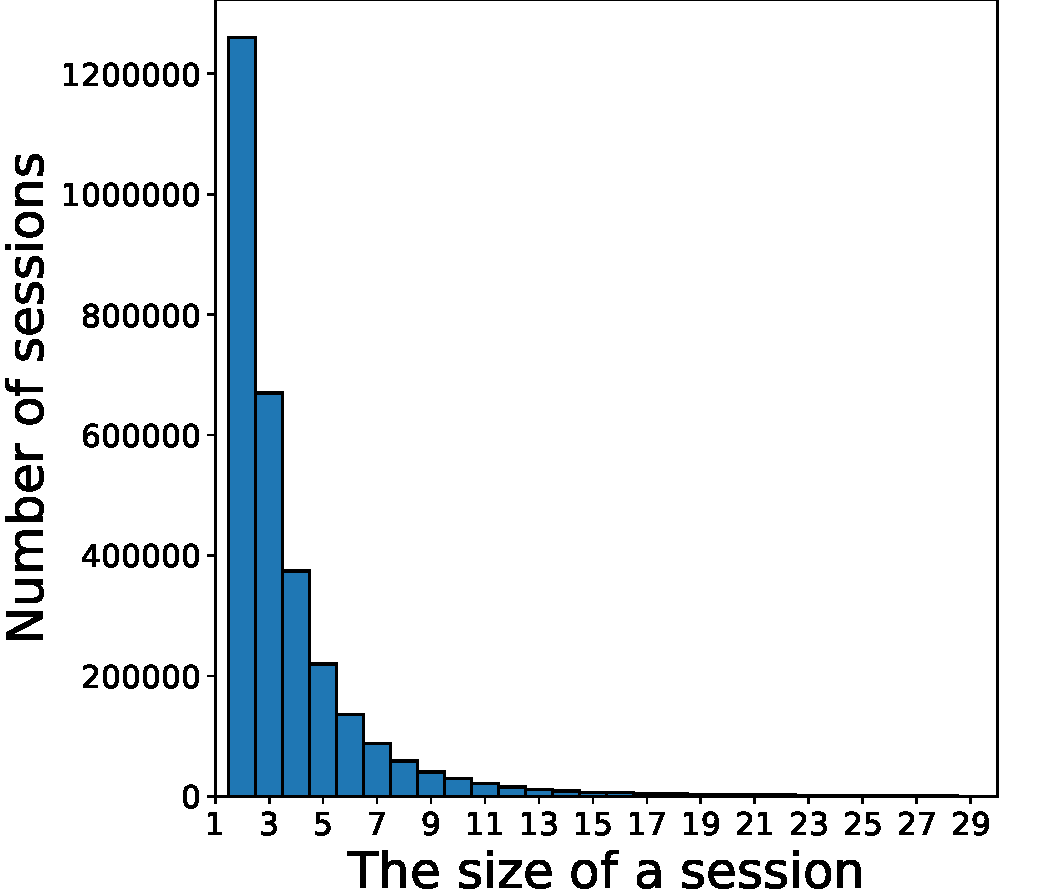
\includegraphics[width=\textwidth]{fig/data_distribution_a.pdf}
        \caption{The histogram of session size, and here the size means the number of clicks (also called user interactions) in one session.}
    \end{subfigure}
    \quad
    \begin{subfigure}[t]{0.3\textwidth}
        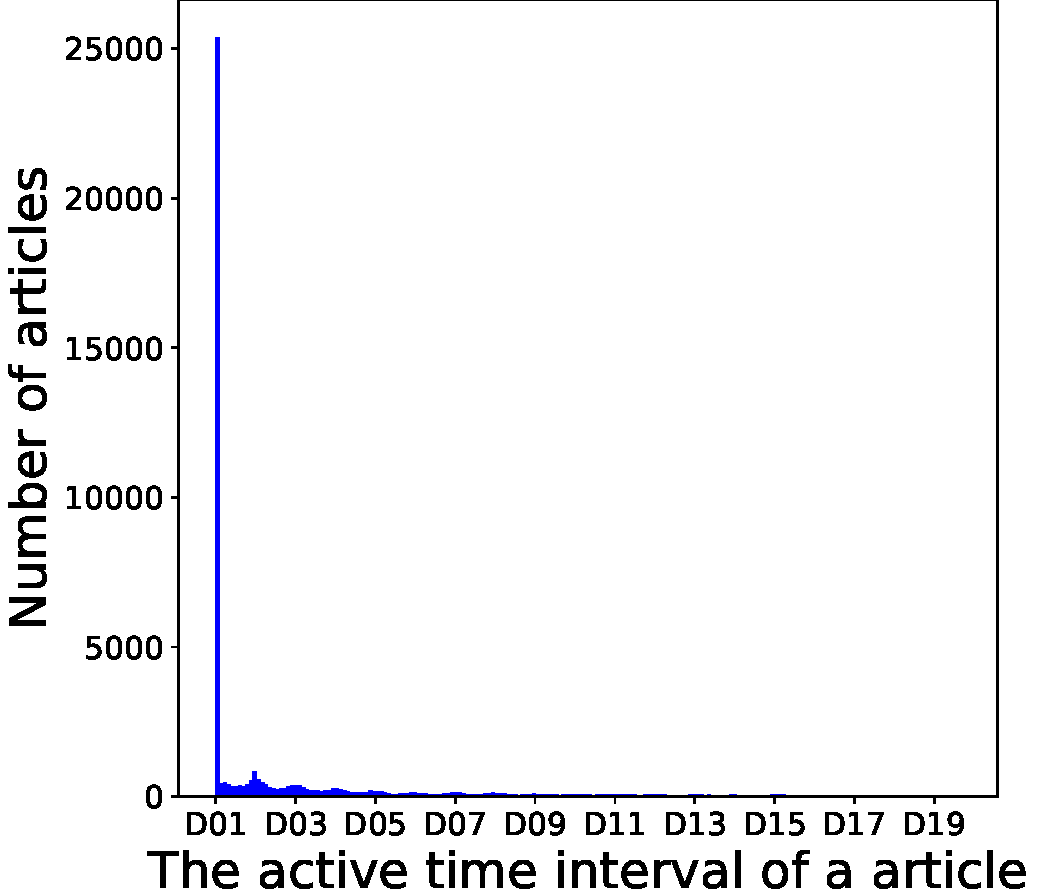
\includegraphics[width=\textwidth]{fig/data_distribution_b.pdf}
        \caption{The histogram of article active time interval, where the the horizontal axis is the relative time (days) between the first click and the last click of a article.}
    \end{subfigure}
    \quad
    \begin{subfigure}[t]{0.3\textwidth}
        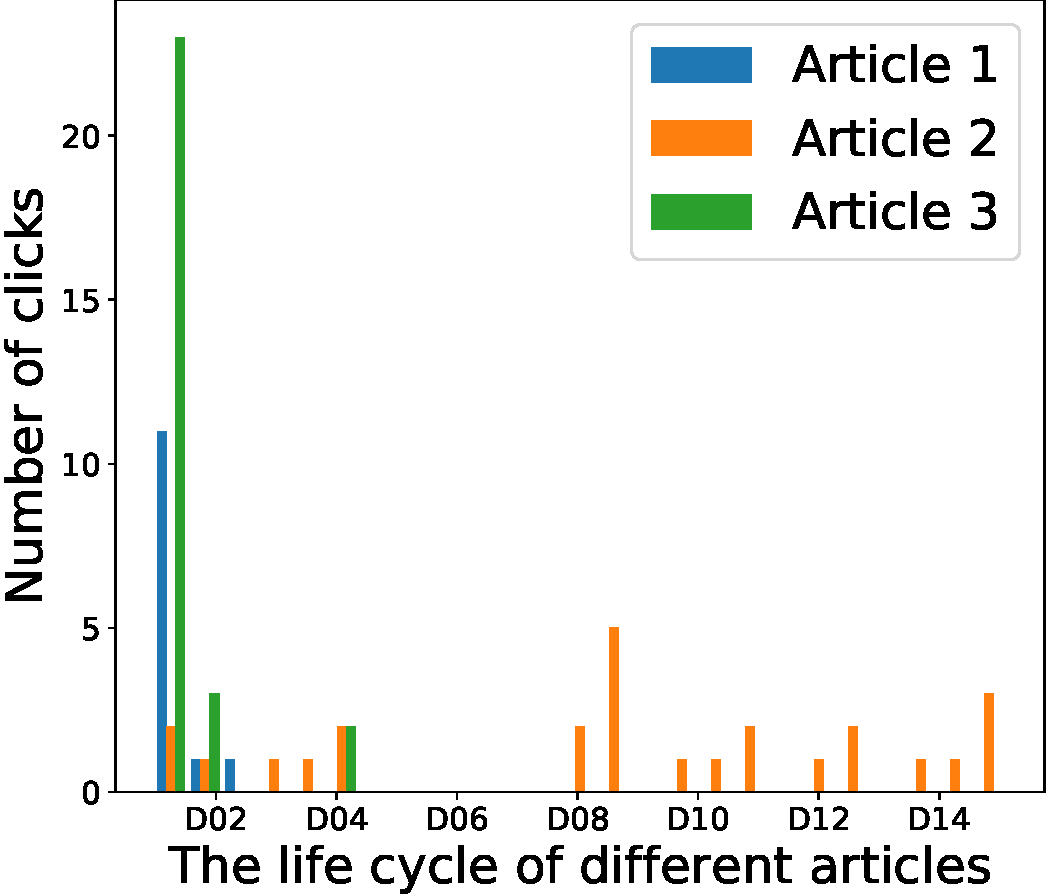
\includegraphics[width=\textwidth]{fig/data_distribution_c.pdf}
        \caption{The illustration of click tendencies drifting with time for different articles, where the horizontal axis is the relative time (days) since the article is published.}
    \end{subfigure}
    \caption{A visual representation of user interactions in the Globo.com dataset. (a) shows the most of sessions are very short, with limited user interactions. (b) shows the most of articles stay active for few time and decay fastly. (c) depicts the activeness of radomly choosed Article 1, 2 and 3, showing that they decay in different mode.}
    \label{fig:data_distribution}
    % \Description[Data distribution]{There're 3 figures to show the data distribution of Globo.com dataset.}
\end{figure*}

Cold-start problem emerges when new users or new articles are introduced into the recommendation system, where users or articles are not seen during the training. While CF and MF methods have difficulty in dealing with this, many hybrid recommendation approaches thus combine content-based method to overcome cold-start problem. 

The temporally ordered user interactions lead to the streaming nature of session data. A session means a sequence of user behaviors takes place within a short time window (e.g. 30 minutes). Therefore it's natural and realistic to formulate the news recommendation task as a session-based sequential recommendation task~\cite{sottocornola2018session,grabe1991current}. As in \figref{fig:representation}, the system yields the next article prediction immediately after the user browses several pieces of news. 
Among most of session-based recommendation approaches, some works show the significant of the temporal information~\cite{garg2019sequence,rakkappan2019context,xu2019time}, but little attention has been paid to different life cycles of items. For example, there are two 3-day-old articles, one is economic article which has lost its effectiveness, another is opinion article and still stay active after 2 days. Clearly, these two articles are weighted differently and this difference should be better made use of to capture the short term preference of user. Besides, following the idea of CF, if two sessions are close in time, the items within these two sessions are more likely to correlated, which is regarded as inter-session temporal information.

Thus, in this paper, we formulate a sequential prediction task and to predict the next item for each new session. We group the age of articles and in-session click time of articles together as intra-session temporal information and consider inter-session temporal information when generate candidate articles. We design a session-based news recommendation system to reconstruct the short term intentions. First, we train a classifier to obtain the article embedding vector (see \secref{sec:3.1}), then we feed article features sequentially into a multi-head attention transformer. Meanwhile, we apply multi-head attention transformer to encode intra-session temporal information, and we multiply sequential article features by the encoded temporal feature as time decay factor (see \secref{sec:3.2}). Through this, we try to extract temporal information of each user interaction, and apply different time decay factors to articles with different life cycles. Third, after embedding, by replacing the last clicked article with negative samples, we can train a classifier to distinguish the truly clicked article from non-clicked articles. Instead of randomly sampling from article database, we consider inter-session temporal information to locate time-aware k-nearest neighbors, and sample negative articles with high similarity (see \secref{sec:3.3}). 

Our contributions are:
\begin{itemize}
    \item We design a time-aware and context-aware news recommendation system, focus on the next-item-prediction problem and articles-cold-start problem.
    \item We highlight that considering intra-session and inter-session temporal information can obtain competitive results. 
    \item We conduct a series of experiments on three real-world news recommendation datasets to show our methods outperform state-of-the-art session-based news recommendation systems.
\end{itemize}

This work is also suitable for other streaming-like scenarios such as tweet-like social media sites~\cite{kwak_what_2010} and E-commerce recommendation~\cite{li_learning_2018}. In some cases, the recommendation system has chances to get user's long-term history by trace user's identification via log-ins or cookies. Even in these cases, how to capture the shifting of short-term interests in real-time is still indispensable.

\begin{figure}[th]
    \centering
    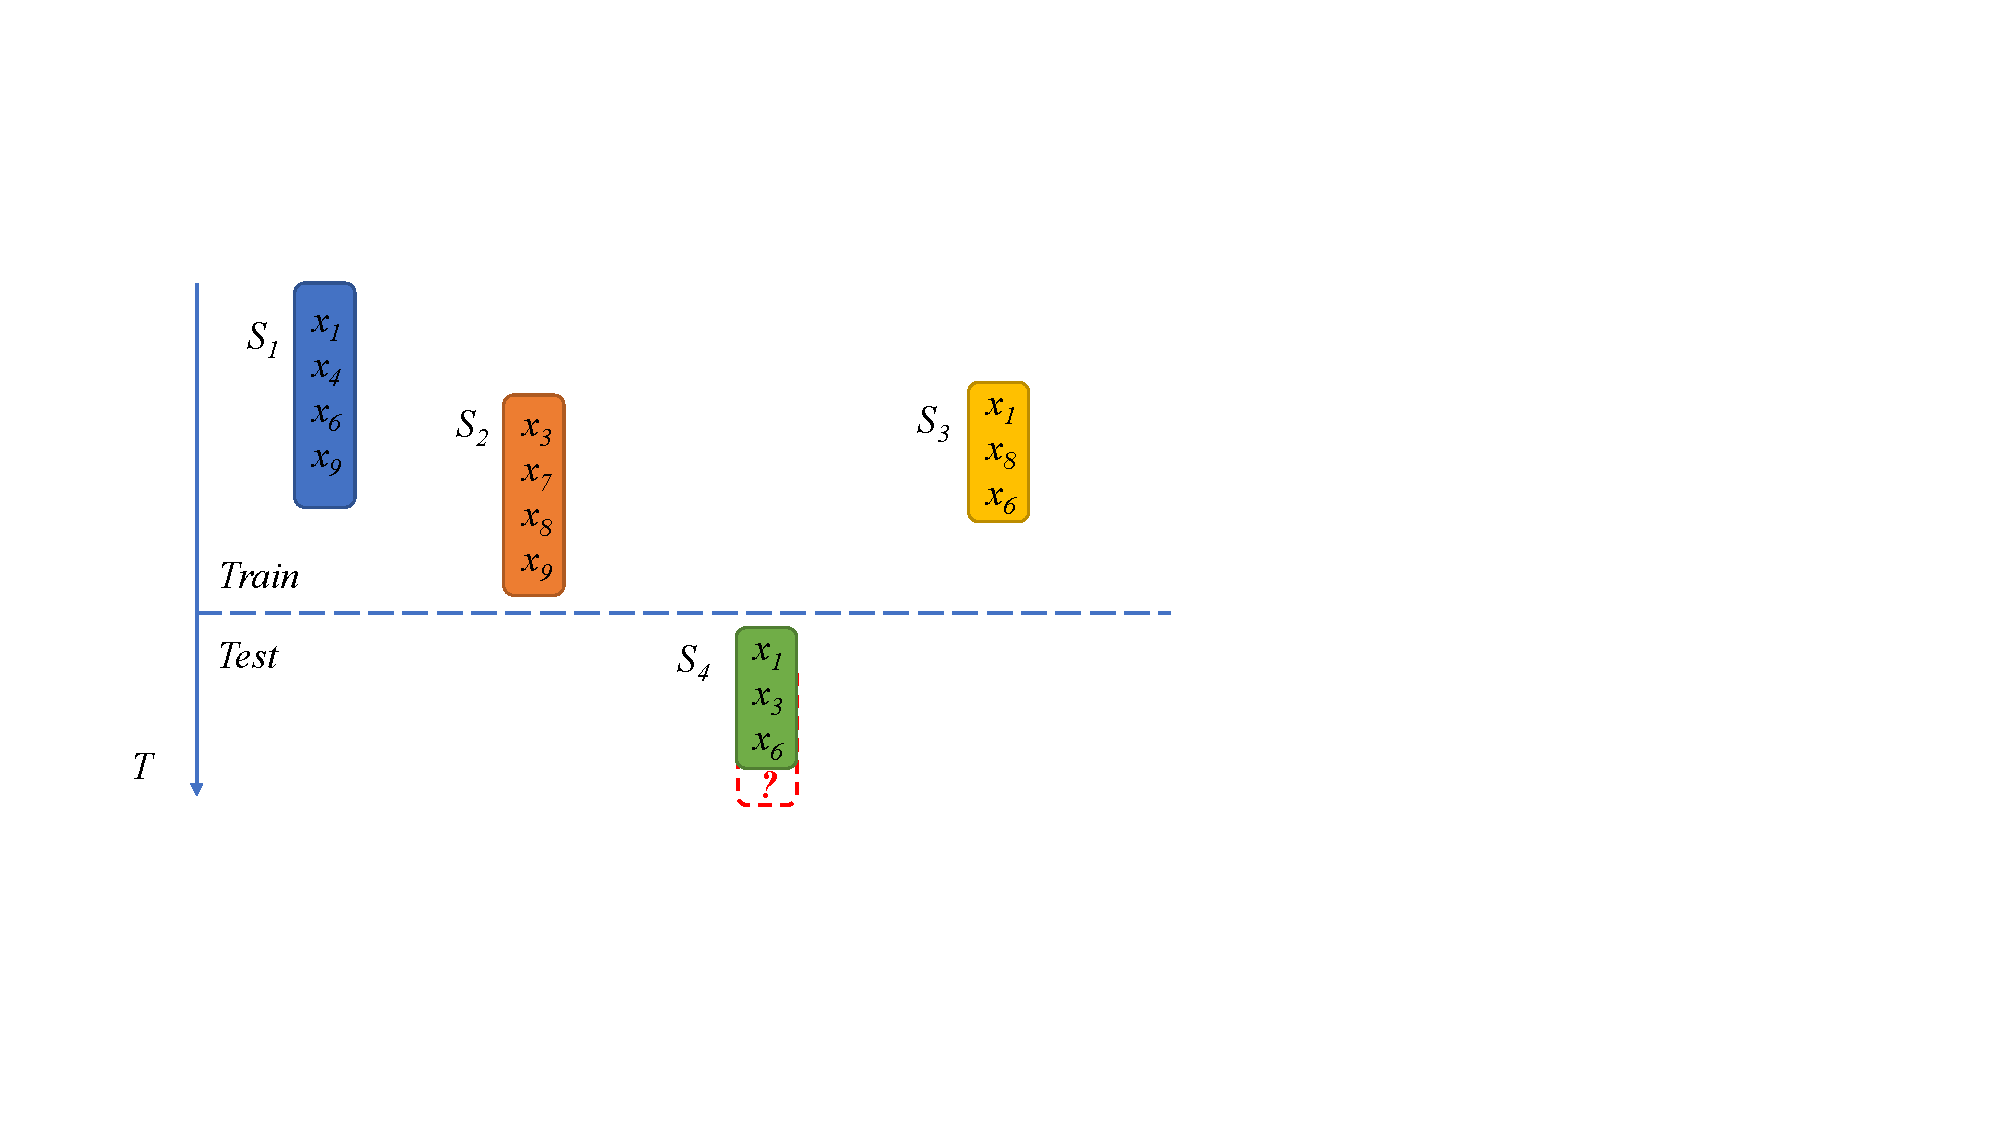
\includegraphics[width=0.9\columnwidth]{fig/example.pdf}
    \caption{A visual representation of session-based news recommendation. $x_i$'s are the news articles consumed by different users in a session $S_j$. The task addressed in this work is next-item prediction for users sessions.}
    \label{fig:representation}
    % \Description[A visual representation]{This is a visual representation of session-based news recommendation}
\end{figure}
